C is the grandad of most of the languages we use today. It's so good that people still use it to create the glorious Linux operating system. So, let's C what it can do!
\\
\\
\textbf{Additional Notes}\\
CHammond made some decent notes on most of this stuff if you want a quick but thorough overview of the module. Check them out on Google Drive if you have access, here: \url{https://docs.google.com/document/d/1t2VUYKYipdOwf7I22OtLSfnoMIe7KPTwmSjbXqMY5FI/edit}

\section{Basics}
C is an \gls{imperative} language, which means that you write programs by saying "do this!" then "do that!". Things get a little more complex than that when you're dealing with bigger programs (Linux kernel, anyone?) but essentially that's what it's about. Here's a quick rundown of things you can do.

\subsection{Variables}
\Glspl{variable} are like, super important. They are the bread and butter of imperative programming, they are ways of storing values so that you can use them again or manipulate them however you desire. Let's look at a few different variable types and how you can define them. I'll also point out here that comments (notes you can add to the code that have no effect on the running) look like \texttt{/* this */} or like \texttt{// this}.
\begin{lstlisting}[language=C]
// Integers (whole numbers)
int someNumber = 42; // yer standard integer, 16 bits in size.
short yolo = 256; // a smaller integer.
char hiya = 25; // a very small integer, range of -127 to +127 makes it awesome for text characters.
long bigNum = 5484198; // For when you want to store biiiig numbers.

// Floating point numbers (numbers with decimal points)
float someNum = 3.4;  // single-precision, 32-bits.
double preciseNum = 3.232365;  // double-precision (durr)

bool amIRetakingTheYear = true;  // true or false, you need stdbool.h though.
\end{lstlisting}

Hey look at that, you can write C! To define a variable, you add the type you want in front of the name you're going to give it. You can then, if you want, assign it a value with the assignment (\texttt{=}) operator, or just leave it. To then access that variable or its value again, you only need its name.

\subsection{Simple Operations}
Operations are built-in mathsy things you can perform on variables. Here's a few you can do:
\subsubsection{Assignment}
Sets the value of a variable.
\begin{lstlisting}[language=C]
    lecturesMissed = 5;
\end{lstlisting}

\subsubsection{Addition}
Adds two numbers together. You can also just add a number on by combining this with the assingment operator.
\begin{lstlisting}[language=C]
    someStupidExample = 4 + 8; // is now 12.
    someStupidExample += 5;  // someStupidExample = 12 + 5 = 17.
\end{lstlisting}

\subsubsection{Subtraction}
Works \textbf{exactly the same} as addition, just with a minus (\texttt{-}) sign instead of a plus sign. Yes, this is starting to bore me now.

\subsubsection{Increment and Decrement}
You can add or subtract a single value with these. You have the choice of applying them before (prefix) or after (suffix). Check this:
\begin{lstlisting}[language=C]
    int some_num = 10;
    some_num++;  // some_num is now 11
    ++some_num;  // some_num is now 12
    some_num--;  // some_num is now 11
\end{lstlisting}

But why do you get the two separate ways of incrementing or decrementing numbers? It's because, when used in an expression, the prefix operator will use the new value in the expression, whereas the postfix will not. Let's see an example because my explanation is kinda bad.
\begin{lstlisting}[language=C]
    int i = 10;
    int k = ++i; // i = 10 + 1 = 11, THEN k = i = 11;
    int k = i++; // k = i = 11, THEN i = 11 + 1 = 12;
\end{lstlisting}
This is the cause of both misery and joy in my opinion. Use it at your own risk.

\subsubsection{Multiplication}
Again, works just like addition but with an asterisk (\texttt{*}).
\begin{lstlisting}[language=C]
    imBored = 5 * 12;  // is now 60.
\end{lstlisting}

\subsubsection{Division}
Hey, guess what? It works in EXACTLY THE SAME WAY. Honestly, I should be getting money for this. But what I will point out is that dividing an integer by an integer returns the whole part of a result, not rounded.
\begin{lstlisting}[language=C]
    int x = 5;
    int y = 2;
    x = x / y;  // x is now 2.
\end{lstlisting}

\subsubsection{Modulo}
It's very possible to get the remainder of dividing integers in C, you must use the modulo or remainder operator.
\begin{lstlisting}[language=C]
    ex = 5 % 2;  // 1, 5/2 is 2.5 or 2 with 1 left over
\end{lstlisting}

\subsubsection{Pointer (De)reference}
Woah there friend, you may need to slow down!

\subsection{Order Of Operations}
Pretty much 100\% confirmed as the first question in the exam. Like in real world maths, operators in C follow a 'precedence', e.g. some are always performed before others. This is known as order of operations, or operator precedence. It goes like this:
\begin{itemize}
    \item \textbf{1 (first)} - postfix increment/decrement, brackets etc.
    \item \textbf{2} - prefix increment/decrement, pointer stuff
    \item \textbf{3} - multiplication, division, modulo
    \item \textbf{4} - addition, subtraction
    \item \text{...} - a bunch of stuff that may not be so important right now.
\end{itemize}
Thanks, \url{http://en.cppreference.com/w/c/language/operator_precedence}.

\subsection{Arrays}
An array is a list of variables for which each have its own index. Basically, when you make your array, you get a big chunk of memory where you can store $n$ number of values... so naturally you can't change its size since that would be a shambles. But rather than try to explain memory voodoo to you, I'll leave that for later and just show you an example of how arrays work.

You define an array similarly to variables, except you're also providing a size.
\begin{lstlisting}[language=C]
    int someList[30];

    // let's give a list values!
    int anotherList[5] = {1, 3, 5, 6, 8};
\end{lstlisting}

It's probably best to think of arrays as like pigeon holes, where the number on the box is how you can refer to it.

\begin{figure}[h]
    \centering
    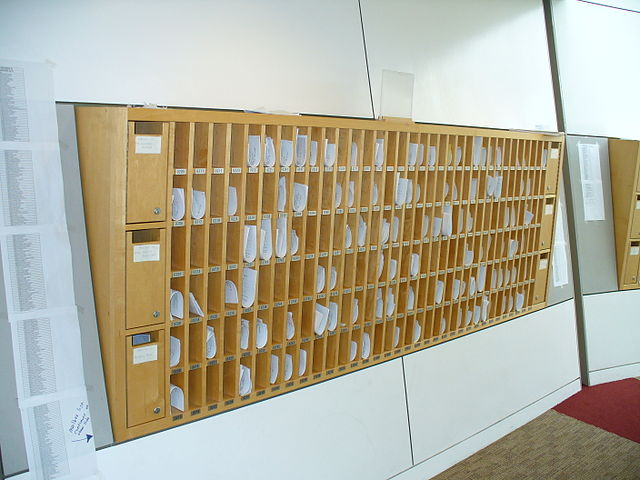
\includegraphics[width=0.5\textwidth]{pigeonhole}
    \caption{A pigeon hole. By "Stacalusa" on Wikipedia.}
\end{figure}

You can reference an item in the array just like any other variable, you just type \texttt{myArray[x]}, where \texttt{x} represents the index of the item (arrays count from 0 though, so beware!).

Since you can have arrays of any type (as long as each item has the same type as each other), you can actually have arrays of arrays, or 2-d arrays. They are simply defined like so:
\begin{lstlisting}[language=C]
    int some_2d_array[3][3] = {
        {1, 2, 3},
        {4, 5, 6],
        {7, 8, 9}
    };

    some_2d_array[1][2] = 4;
\end{lstlisting}

Oh oops, maybe I should point out at the same time that text is represented in C using \glspl{string}, which are quite literally an array of characters. Here's the difference though. You can define \gls{constant} strings (value doesn't change), by using this funky pointer notation (it will be explained later): \texttt{char *my\_string = "Dat boi";} They can also be represented with your standard ol' \texttt{char meme[10]} or whatever. Another difference is that strings have a hidden character at the end to say that the string is finished, called a 'null' character. It's represented as \texttt{\textbackslash0} and literally serves no other purpose.

\subsection{Call functions}
C comes with a bunch of \glspl{functions} which are blocks of code which do things. Some functions take in values and some return values, which makes them really handy for not writing the same damn piece of code a million times over. Most of them require you to import the related code \gls{library} to your program. You can do this like so, at the beginning of your file:

\begin{centering}
    \texttt{#include <stdlib.h>} - include a built-in library called "stdlib".\\
    \texttt{#include "mylib.h"} - include a library that is stored in the same directory which is called "mylib.h".\\
    \texttt{#include "libs/somelib.h"} - include a library that is stored in a directory called "libs".
\end{centering}

There's a couple of neat ones that you won't go wrong with remembering. They may come back when you least expect it!
\begin{itemize}
    \item \textbf{stdlib.h} - the 'standard' library which contains things like memory allocation, and value conversion (based \texttt{atoi()}, thank you).
    \item \textbf{stdio.h} - input/output library. Expect things like printing to console (\texttt{printf()}) as well as reading, along with file stuff too.
    \item \textbf{string.h} - helpful string library, which contains a bunch of helper functions such as comparing strings (\texttt{strcmp()}) and so on.
    \item \textbf{stdbool.h} - allows you to use the \texttt{bool} type, which is just true/false.
    \item \textbf{math.h} - this will save your butt, as well as containing mathsy things like trigonometry functions, you also get some neat constants like \texttt{M\_PI} which gives you Pi. Awesome!
\end{itemize}

\subsection{User-Defined Functions}
So, you want to make your own functions, huh? Very well. Functions are defined with, in order: the return variable type, the function name, as well as its \glspl{parameter} (if any), followed by the content of the function. Let's look at an example, we'll call it matt, and it will take an integer, add 5, and return it.
\begin{lstlisting}[language=C]
    int matt(int input) {
        input += 5;
        return input;
    }
\end{lstlisting}

That wasn't too bad was it? Note the "return" keyword. What this does is that it returns whatever you put after it. In this case, it's returning the value of \texttt{input}. This doesn't have to be a variable; if you had a function called \texttt{give\_me\_lemon} for instance, you could always have \texttt{return "lemon";} Also note that for each parameter, you need to provide its type. Very important.

Every program in C must have a main function, which returns either an \texttt{int} or \texttt{void}. Void is a magic keyword that means, "this function does not return anything". The main function is the entry point, the way in, to your program. Set things up there, I recommend.

\subsection{If Statements And Logic}
Maybe there's some code you don't want to run all the time. If statements are your solution!
\begin{lstlisting}[language=C]
    if (logical_statement) {
        do_something();
    }
    else if (another_statement) {
        do_something_else();
    }
    else {
        give_up();
    }
\end{lstlisting}
